% !TeX program = pdfLaTeX
\documentclass[12pt]{article}
\usepackage{amsmath}
\usepackage{graphicx,psfrag,epsf}
\usepackage{enumerate}
\usepackage{natbib}
\usepackage{textcomp}
\usepackage[hyphens]{url} % not crucial - just used below for the URL
\usepackage{hyperref}
\providecommand{\tightlist}{%
  \setlength{\itemsep}{0pt}\setlength{\parskip}{0pt}}

%\pdfminorversion=4
% NOTE: To produce blinded version, replace "0" with "1" below.
\newcommand{\blind}{0}

% DON'T change margins - should be 1 inch all around.
\addtolength{\oddsidemargin}{-.5in}%
\addtolength{\evensidemargin}{-.5in}%
\addtolength{\textwidth}{1in}%
\addtolength{\textheight}{1.3in}%
\addtolength{\topmargin}{-.8in}%

%% load any required packages here
\usepackage{amssymb, amsmath, mathtools, dsfont, bbm, array, booktabs} \usepackage[ruled,vlined, linesnumbered]{algorithm2e}




\begin{document}


\def\spacingset#1{\renewcommand{\baselinestretch}%
{#1}\small\normalsize} \spacingset{1}


%%%%%%%%%%%%%%%%%%%%%%%%%%%%%%%%%%%%%%%%%%%%%%%%%%%%%%%%%%%%%%%%%%%%%%%%%%%%%%

\if0\blind
{
  \title{\bf Visual diagnostics for constrained optimisation with application to guided tours}

  \author{
        Author 1 \thanks{The authors gratefully acknowledge \ldots{}} \\
    Department of YYY, University of XXX\\
     and \\     Author 2 \\
    Department of ZZZ, University of WWW\\
      }
  \maketitle
} \fi

\if1\blind
{
  \bigskip
  \bigskip
  \bigskip
  \begin{center}
    {\LARGE\bf Visual diagnostics for constrained optimisation with application to guided tours}
  \end{center}
  \medskip
} \fi

\bigskip
\begin{abstract}
Friedman \& Tukey commented on their initial paper on projection pursuit in 1974 that ``the technique used for maximising the projection index strongly influences both the statistical and the computational aspects of the procedure.'' While many projection pursuit indices have been proposed in the literature, few concerns the optimisation procedure. In this paper, we developed a system of diagnostics aiming to visually learn how the optimisation procedures find its way towards the optimum. This diagnostic system can be applied more generally to help practitioner to unveil the black-box in randomised iterative (optimisation) algorithms. An R package, ferrn, has been created to implement this diagnostic system.
\end{abstract}

\noindent%
{\it Keywords:} optimisation, projection pursuit, guided tourr, visual, diagnostics, R
\vfill

\newpage
\spacingset{1.45} % DON'T change the spacing!

\hypertarget{introduction}{%
\section{Introduction}\label{introduction}}

Visualisation has been widely used in exploratory data analysis. Presenting information in a graphical format often allows people to see information they would otherwise not see. This motivates our work of creating plots to diagnose optimisation algorithms in the context of projection pursuit guided tour, with the aim to understand and compare features of different existing algorithms.

In an optimization problem the goal is to find the best solution within the space of all feasible solutions which typically is represented by a set of constraints. The problem consists in optimizing an objective function \(f: S \rightarrow \mathbb{R}\) with \(S \in \mathbb{R}^n\) in a reduced space given by the problem constraints to either minimize or maximize a function.

Projection pursuit and guided tour are exploratory data analysis tools that detect interesting structure of high dimensional data through projection on low dimensional space. Optimisation is applied here to search for the low dimensional space that finds the most interesting projection.

The remainder of the paper is organised as follows.
Section \ref{optim} provides a literature review of optimisation methods, specifically the line search methods used in projection pursuit guided tour.
Section \ref{tour} reviews projection pursuit guided tour, forms the optimisation problem, and introduces three main existing algorithms.
Section \ref{vis-diag} presents the new visual diagnostics design, from forming the data object to the definition of different diagnostic plots with some small examples.
Section \ref{application} shows the application of how the diagnostic plots designed in section \ref{vis-diag} can be used to understand and compare different algorithms and how they contribute to modifications that improve the algorithms.
Finally, Section \ref{implementation} describes the R package: ferrn, that implements all the visual diagnostics above.

\hypertarget{optim}{%
\section{Optimisation Methods}\label{optim}}

Given an optimisation problem, two basic approaches find the optimum based on different thinking.
An analytical approach aims to find the optimal solution in a finite number of steps, but a potential issue with it is that the closed-form solution may not be available when the problem starts to become complex.
An iterative approach, on the other hand, finds the optimum based on the idea of making progressive improvement to the current solution. An iterative method may end up finding a local optimum but the progressive nature of the algorithm allows the practitioner to decide when to stop if a desirable accuracy has been achieved.

A traditional while often used in practice is an iterative method called \emph{line search method} \citep{fletcher2013practical}. In a simple one-dimensional problem of finding the \(x\) that minimises \(f(x)\), line search achieves the goal via an iterative algorithm in the form of Equation \ref{eq:line-search}.

\begin{equation}
x^{(j + 1)} = x^{(j)} + \alpha_k* d^{(j)}
\label{eq:line-search}
\end{equation}

where \(d^{(j)}\) is the searching direction in iteration \(j\), and \(\alpha_j\) is the step-size. Strictly speaking, \(\alpha_k\) is chosen by another minimisation of \(f(x^{(j)} + \alpha* d^{(j)})\) with respect to \(\alpha\) and theoretical results have demonstrated the global convergence of the algorithm when the exact minimisation of \(\alpha_j\) is attained \citep{curry1944method}. In practice, this second minimisation is rarely implemented due to its computational demanding or even the existence of such a minimisation. A more realistic approach is to impose a mandatory decrease in the objective function for each iteration: \(f^{(j+1)}> f^{(j)}\) and despite we lose the guarantee on global convergence, this approach turns out to be efficient in practical problems.

\hypertarget{tour}{%
\section{Projection pursuit guided tour}\label{tour}}

Modern development of the line search methods focuses on proposing different computation on the searching direction: \(d^{(j)}\) and various approximations on the step size: \(\alpha_j\) catered for practical optimisation problems. The specific problem context we are interested in is called projection pursuit guided tour.
Projection pursuit and guided tour are two separate methods in exporatory data analysis focusing on different aspects: coined by \citet{friedman1974projection}, projection pursuit detects interesting structures (i.e.~clustering, outliers and skewness) in multivariate data via low dimensions projection; whilst guided tour is a particular variation in a broader class of data visualisation method called tour.

Let \(\mathbf{X}_{n \times p}\) be the data matrix, an n-d projection can be seen as a linear transformation \(T: \mathbb{R}^p \mapsto \mathbb{R}^d\) defined by \(\mathbf{P} = \mathbf{X} \cdot \mathbf{A}\), where \(\mathbf{P}_{n \times d}\) is the projected data and \(\mathbf{A}_{p\times d}\) is the projection basis. Define \(f: \mathbb{R}^{n \times d} \mapsto \mathbb{R}\) to be an index function that maps the projection basis \(\mathbf{A}\) onto an index value \(I\), this function is commonly known as the projection pursuit index (PPI) function, or the index function and is used to measure the ``interestingness'' of a projection. A number of index functions have been proposed in the literature to detect different data structures, including Legendre index \citep{friedman1974projection}, Hermite index \citep{hall1989polynomial}, natural Hermite index \citep{cook1993projection}, chi-square index \citep{posse1995projection}, LDA index \citep{lee2005projection} and PDA index \citep{lee2010projection}.

In their initial paper, \citet{friedman1974projection} noted that ``\ldots{}, the technique used for maximising the projection index strongly influences both the statistical and the computational aspects of the procedure.'' Hence, effective optimisation algorithms are necessary for projection pursuit to find the bases that give interesting projections. While we leave the formal construction of the optimisation problem and existing algorithms to section \ref{tour-optim}, we outline the general idea here. Given a random starting (current) basis, projection pursuit repeatedly searches for candidate bases nearby until it finds one with higher index value than the current basis. In the second round, that basis becomes the current basis and the repetitive sampling continues. The process ends until no better basis can be found or one of the termination criteria is reached.

Before introducing the guided tour, we shall be familiar with the general tour method \citep{cook2008grand}. A tour produces animated visualisation of the high dimensional data via rotating low dimension planes. The smoothness of the animation is ensured by computing a series of intermediate planes between two low dimension planes via geodesic interpolation and we refer readers to \citet{buja2005computational} for the mathematical details. Iteratively choosing different low dimension planes and interpolating between them forms a tour path. Different types of tour methods choose the low dimensional planes differently and we mention two other types of tour that are commonly used. A grand tour selects the planes randomly in the high dimensional space and hence serves as an initial exploration of the data. Manual control allows researches to fine-tuning an existing projection by gradually phase in and out one variable.

Guided tour chooses the planes produced by optimising the projection pursuit index function. Figure \ref{tour-path} shows a sketch of the tour path consisting of the blue frames produced by the projection pursuit optimisation algorithm iteratively and the white frames, which are the interpolations between two blue frames. The tour method has been implemented in the \emph{tourr} package in R, available on the Comprehensive R Archive Network at \url{https://cran.r-project.org/web/packages/tourr/} \citep{wickham2011tourrpackage}.

\begin{figure}

{\centering 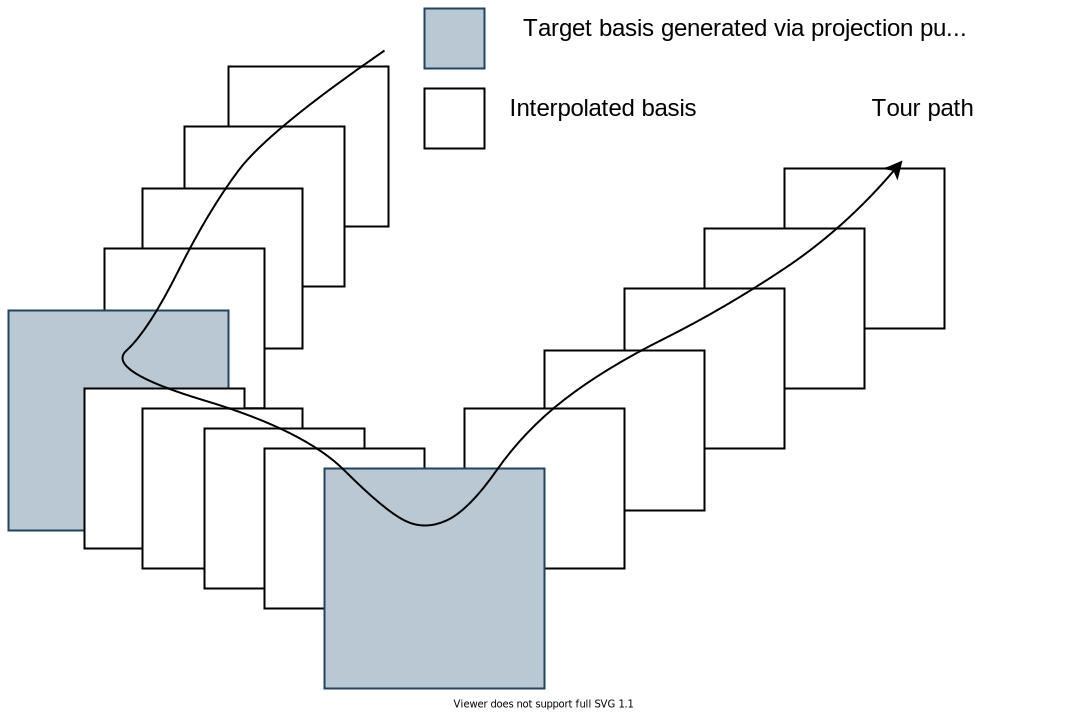
\includegraphics[width=0.6\linewidth,height=0.3\textheight]{/Users/hzha400/Documents/3.PhD/research/paper-tour-vis/img/tour_path} 

}

\caption{Each square (frame) represents the projected data with a corresponding basis. Blue frames have bases found by an optimisation algorithm iteratively whilst the white frames are constructed by geodesic interpolation between two blue frames.}\label{fig:tour-path}
\end{figure}



\hypertarget{tour-optim}{%
\subsection{Optimisation in the tour}\label{tour-optim}}

Now we begin to formulate the optimisation problem. Given a randomly generated starting basis \(\mathbf{A}_1\), projection pursuit finds the final projection basis \(\mathbf{A}_T\) that satisfies the following optimisation problem:

\begin{align}
&\arg \max_{\mathbf{A} \in \mathcal{A}} f(\mathbf{X} \cdot \mathbf{A}) \\
&s.t.  \mathbf{A}^{\prime} \mathbf{A} = I_d
\end{align}

where \(I_d\) is the d-dimensional identity matrix. The constraint requires the projection basis \(\mathbf{A}\) to be an orthogonal matrix with each column vector being orthonormal.

There are several features of this optimisation that are worth noticing. First of all, it is a multivariate constraint optimisation problem. Since the decision variables are the entries of a projection basis, it is required to be orthonormal. It is also likely that the objective function is non-differentiable or the gradient information is simply not available. In this case, we will need to either use some approximation of the gradient or turn to derivative free methods. Given the goal of projection pursuit as finding the basis with the largest index value, the optimisation problem needs to be able to find the global maximum. Along the way, local maximum may also be of our interest since they could present unexpected interesting projections. There is also one computational consideration: the optimisation procedure needs to be easy to compute since the tour animation is played in real-time.

\hypertarget{existing-algorithms}{%
\subsection{Existing algorithms}\label{existing-algorithms}}

Below we introduce three possible algorithms: \texttt{search\_better} and \texttt{search\_better\_random} are derivative free methods that sample candidate bases in the neighbourhood, whilst \texttt{search\_geodesic} is an analogue of gradient ascent on the manifold of the projection basis.

\begin{algorithm}
\SetAlgoLined
  \SetKwInOut{Input}{input}
  \SetKwInOut{Output}{output}
    \Input{$\mathbf{A}_{\text{cur}}$, $f$, $\alpha$, $l_{\max}$} 
    \Output{$\mathbf{A}_{l}$}
  initialisation\;
  Set $l = 1$\;
  \While{$l < l_{\max}$}{
    Generate $\mathbf{A}_{l} = (1- \alpha)\mathbf{A}_{\text{cur}} + \alpha \mathbf{A}_{\text{rand}}$ and orthogonise $\mathbf{A}_{l}$\;
    Compute $I_{l}  = f(\mathbf{A}_{l})$\;
    \If{$I_{l} > I_{\text{cur}}$}{
      \KwRet{$\mathbf{A}_{l}$} \;
      }
    $l = l + 1$\;
  }
  \caption{random search}
  \label{random-search}
\end{algorithm}

\texttt{search\_better} is a random search device that samples a candidate basis \(\mathbf{A}_{l}\) in the neighbourhood of the current basis \(\mathbf{A}_{\text{cur}}\) by \(\mathbf{A}_{l} = (1- \alpha)\mathbf{A}_{\text{cur}} + \alpha \mathbf{A}_{\text{rand}}\) where \(\alpha\) controls the radius of the sampling neighbourhood and \(\mathbf{A}_{\text{rand}}\) is a randomly generated matrix with the same dimension as \(\mathbf{A}_{\text{cur}}\). \(\mathbf{A}_{l}\) is then orthogonalised to ensure the orthonormal constraint is fulfilled. When a basis is found with index value higher than the current basis \(\mathbf{A}_{\text{cur}}\), the search terminates and outputs the basis for guided tour to construct an interpolation path. The next iteration of search begins after adjusting \(\alpha\) by a cooling parameter: \(\alpha_{j+1} = \alpha_j * \text{cooling}\). Another termination condition is when the maximum number of iteration \(l_{\max}\) is reached. A slightly different cooling scheme has been proposed by \citet{posse1995projection} to include a halving parameter \(c\). Rather than reducing the radius of the searching neighbourhood, \(\alpha\), at each iteration, Posse's design only adjust \(\alpha\) if the last search takes more than \(c\) times to find an accepted basis to avoid the searching space being reduced too fast. The algorithm of \texttt{search\_better} is summarised in Algorithm \ref{random-search}. {[}mention orthonormalise to ensure the constraint is fulfilled; don't use derivative information but a random search{]}

\begin{algorithm}
\SetAlgoLined
    Compute $I_{l} = f(\mathbf{A}_{l})$ and $T(l) = \frac{T_0}{\log(l + 1)}$\;
      \eIf{$I_{l} > I_{\text{cur}}$}{
        \KwRet{$\mathbf{A}_{l}$} \;
      }{
        Compute $P= \min\left\{\exp\left[-\frac{I_{\text{cur}} -I_{l}}{T(l)}\right],1\right\}$\;
        Draw $U$ from a uniform distribution: $U \sim \text{Unif(0, 1)}$\;
        \If{$P > U$}{
           \KwRet{$\mathbf{A}_{l}$} \;
        }
      }
  \caption{simulated annealing}
  \label{simulated_annealing}
\end{algorithm}

Simulated annealing \citep[\citet{bertsimas1993simulated}]{kirkpatrick1983optimization} uses the same sampling process as \texttt{search\_better} but allow a probabilistic acceptance of a basis with lower index value based on a cooling scheme \(T(l)\). Given an initial \(T_0\), the temperature at iteration \(l\) is defined as \(T(l) = \frac{T_0}{\log(l + 1)}\). When a candidate basis fails to have an index value larger than the current basis, simulated annealing gives it a second chance to be accepted with probability \[P= \min\left\{\exp\left[-\frac{I_{\text{cur}} - I_{l}}{T(l)}\right],1\right\}\] where \(I_{(\cdot)}\) denotes the index value of a given basis. This implementation allows the algorithm to jump out of a local maximum and enables a more holistic search of the whole parameter space. This feature is particularly useful when the dimension of the projected space is smaller than the number of informative variables in the dataset (i.e.~a one dimensional projection of the dataset with two informative variables). The algorithm can be written as replacing line 5-8 of Algorithm \ref{random-search} with Algorithm \ref{simulated_annealing}.

\begin{algorithm}
\SetAlgoLined
\SetKwInOut{Input}{input}
  \SetKwInOut{Output}{output}
    \Input{$\mathbf{A}_{\text{cur}}$, $f$, $l_{\max}$, $n = 5$, $\delta$}
    \Output{$\mathbf{A}_{**}$}
  initialisation\;
  Set $l = 1$\;
  \While{$l < l_{\max}$}{
    Generate $2n$ bases in a small neighbourhood, $\delta$, of $\mathbf{A}_{\text{cur}}$ and ensure orthogonality \;
    Find the one with the largest index value: $\mathbf{A}_{*}$\;
    Construct the geodesic $\mathcal{G}$ from $\mathbf{A}_{\text{cur}}$ to $\mathbf{A}_{*}$\;
    Optimise the index value on the geodesic $\mathcal{G}$ over a 90 degree window to produce the optima $\mathbf{A}_{**}$  \;
    Compute $I_{**} = f(\mathbf{A}_{**})$, $p_{\text{diff}} = (I_{**} - I_{\text{cur}})/I_{**}$\;
      \If{$p_{\text{diff}} > 0.001$}{
         \KwRet{$\mathbf{A}_{**}$} \;
      }
    $l = l + 1$\;
  }
  \caption{search geodesic}
  \label{search-geodesic}
\end{algorithm}

\citet{cook1995grand} used a gradient ascent algorithm on the manifold of the projection bases. In gradient ascent, one first find the direction for improvment via computing the gradient information. In \texttt{search\_geodesic}, \(2n\) bases are first generated in a tiny neighbourhood of the current basis, controlled by the neighbourhood parameter \(\delta\). A geodesic is then constructed using the current basis and one of the \(2n\) bases that have the highest index value. If the neighbourhood parameter \(\delta\) is tiny, the geodesic constructed is an analogue of the gradient information in the curved space and can work as the searching direction. In gradient ascent, the next step is to conduct a line search to find the best improvement along the gradient direction. In \texttt{search\_geodesic}, this step is replaced by optimising the index value along the geodesic direction constructed before over an 90 degree angle from \(-\pi/4\) to \(\pi/4\). The optima \(\mathbf{A}_{**}\) is outputted for the current iteration if the percentage change in the index value between \(\mathbf{A}_{**}\) and \(\mathbf{A}_{\text{cur}}\) is greater than a threshold value. As above, another termination condition is when \(l_{\max}\) is reached. Algorithm \ref{search-geodesic} summarises the steps in geodesic search.

\hypertarget{vis-diag}{%
\section{Visual diagnostics}\label{vis-diag}}

To be able to make diagnostic plot, the optimisation algorithm should populate a data structure that contains the key elements of the algorithm. When the algorithm runs, key information regarding the decision variable, objective function and hyper-parameters needs to be recorded and stored as a data object for future analysis.

\hypertarget{data-structure-for-diagnostics}{%
\subsection{Data structure for diagnostics}\label{data-structure-for-diagnostics}}

In the optimisation algorithms for projection pursuit, three main elements to record are 1) projection bases: \(\mathbf{A}\), 2) index values: \(I\), and 3) State: \(S\), which labels the observation with detailed stage in the optimisation. Multiple iterators are also needed to index the data collected at different levels. \(t\) is a unique identifier that prescribes the natural ordering of each observation; \(j\) is the counter for each search-and-interpolate round, which remains the same within one round and has an increment of one once a new round starts. \(l\) is the counter for each search/interpolation allowing us to know how many basis the algorithm has searched before finding one to output. There are other parameters that are of our interest and we denote them as \emph{\(V_{p}\)}. In projection pursuit, this includes \(V_1 = \text{method}\), which tags the name of the algorithm used and \(V_2 = \text{alpha}\), the neighbourhood parameter that controls the size in sampling candidate bases. A matrix notation of the data structure is presented in Equation \ref{eq:data-structure}.

\begin{equation}
\left[
\begin{array}{c|ccc|cc|cc}
t & \mathbf{A} & I & S & j &  l  & V_{1} & V_{2}\\
\hline
1 & \mathbf{A}_1 & I_1 & S_1 & 1 & 1 & V_{11} & V_{12}\\
\hline
2 & \mathbf{A}_2 & I_2 & S_2 & 2 & 1  & V_{21}  & V_{22}\\
3 & \mathbf{A}_3 & I_3 & S_3 & 2 & 2  & V_{31}  & V_{32}\\
\vdots & \vdots &\vdots &\vdots  &\vdots & \vdots &\vdots  &\vdots\\
\vdots & \vdots & \vdots &\vdots & 2 & l_2 & \vdots  & \vdots\\
\hline
\vdots &\vdots & \vdots &\vdots & 2  & 1& \vdots & \vdots\\
\vdots &\vdots &\vdots &\vdots & 2 & 2& \vdots &  \vdots\\
\vdots &\vdots &\vdots &\vdots &\vdots & \vdots & \vdots  &\vdots \\
\vdots &\vdots &\vdots &\vdots & 2 & k_2 &\vdots  & \vdots\\
\hline
\vdots &\vdots &\vdots &\vdots &\vdots & \vdots &\vdots &\vdots \\
\hline
\vdots & \vdots & \vdots &\vdots  & J &  1 & \vdots & \vdots \\
\vdots &\vdots &\vdots &\vdots &\vdots & \vdots &\vdots &\vdots \\
T & \mathbf{A}_T & I_T &S_T  & J &  l_{J} & V_{T1}& V_{T2}\\
\hline
\vdots &\vdots & \vdots &\vdots & J  & 1& \vdots & \vdots\\
\vdots &\vdots &\vdots &\vdots &\vdots & \vdots & \vdots  &\vdots \\
\vdots &\vdots &\vdots &\vdots & J & k_J &\vdots  & \vdots\\
\hline
\vdots& \vdots & \vdots & \vdots & J+1 & 1 & \vdots& \vdots\\
\vdots &\vdots &\vdots &\vdots &\vdots & \vdots &\vdots &\vdots \\
T^\prime & \mathbf{A}_{T^\prime} & I_{T^\prime} &S_{T^\prime}  & J+1 &  l_{J+1} & V_{T^\prime 1}& V_{T^\prime 2}\\
\end{array}
\right]
= 
\left[
\begin{array}{c}
\text{column name} \\
\hline
\text{search (start basis)} \\
\hline
\text{search} \\
\text{search} \\
\vdots \\
\text{search (accepted basis)} \\
\hline
\text{interpolate} \\
\text{interpolate} \\
\vdots \\
\text{interpolate} \\
\hline
\vdots \\
\hline
\text{search} \\
\vdots \\
\text{search (final basis)} \\
\hline
\text{interpolate} \\
\vdots \\
\text{interpolate} \\
\hline
\text{search (no output)} \\
\vdots \\
\text{search (no output)} \\
\end{array}
\right]
\label{eq:data-structure}
\end{equation}

where \(T^{\prime} = T + k_{J}+ l_{J+1}\). Note that we deliberately denote the last round of search as \(j = J+1\) and in that round there is no output/interpolation basis and the algorithm terminates. This notation allows us to denote the last complete search-and-interpolate round as round \(J\) and hence the final basis is \(A_T\) and highest index value found is \(I_T\).

It is worth noticing that the data structure constructed above meets the tidy data principle \citep{wickham2014tidy} that states

\begin{enumerate}
\def\labelenumi{\arabic{enumi})}
\tightlist
\item
  each observation forms a row,
\item
  each variable forms a column, and
\item
  each type of observational unit forms a table
\end{enumerate}

The wrangling and visualisation of tidy data have been greatly simplified by the well-known dplyr\citep{dplyr} and ggplot2\citep{ggplot2} package.

With a constructed data object, the construction of diagnostic plots is inspired by the concept of grammar of graphic \citep{wickham2010layered}, which powers the primary graphical system in R, ggplot2 \citep{ggplot2}. In grammar of graphic, plots are not defined by its appearance (i.e.~boxplot, histogram, scatter plot etc) but by ``stacked layers''. Using this design, ggplot does not have to develop a gazillion of functions that each produces a different type of plot from a different data structure. Instead, it aesthetically maps variables (and its statistical transformation) in a dataset to different geometric objects (points, lines, box-and-whisker etc) and builds the plot through overlaying different layers.

\hypertarget{check-how-hard-the-optimiser-is-working}{%
\subsection{Check how hard the optimiser is working}\label{check-how-hard-the-optimiser-is-working}}

A primary interest of diagnosing an optimisation algorithm is to study how it progressively finds its optimum. One way of doing it is to plot the index value across its natural ordering \(t\), however, it usually takes the algorithm much longer to find a better basis than the current one towards the end of the search.
When plotting the searching observations as points in a plot, the space each iteration takes will be proportional to the number of points in that iteration.

Another option is to use summarisation for each iteration. Boxplot is a suitable candidate that provides five points summary of the data, however, there are two pieces of information missing from the boxplot: 1) It does not report the number of points, and 2) the position of the last basis. This could be remedied by adding more layers using the concept of grammar of graphics. A label geometry is added at the bottom of the plot to show the number of points in each iteration and a line geometry links the last basis in each iteration. Further, an option to switch between displaying points and boxplot geometry is helpful since point geometry can be more intuitive for the iteration with few observations. This is achieved via a \texttt{cutoff} parameter.

Figure \ref{fig:toy-search} presents a comparison between the two plotting options discussed above. Using the natural order to plot searching points distorts the point from the first few iterations and over-emphasizes the searches in the last few iterations. The second plot design evenly presents the summarised information for each iteration while allowing for a switch to the full information for the iteration with small number of observations.

\begin{figure}

{\centering \includegraphics{/Users/hzha400/Documents/3.PhD/research/paper-tour-vis/figs/toy-search-1} 

}

\caption{A comparison of \texttt{search\_better} with different parameter value on \texttt{max\_tries}. A switch of geometry from points to boxplot happens when the count in the iteration excess 15 to avoid overplotting. With \texttt{max\_tries\ =\ 500} specification, the algorithm is working much harder towards to the end.}\label{fig:toy-search}
\end{figure}



\hypertarget{examining-the-optimisation-progress}{%
\subsection{Examining the optimisation progress}\label{examining-the-optimisation-progress}}

\begin{figure}

{\centering \includegraphics{/Users/hzha400/Documents/3.PhD/research/paper-tour-vis/figs/toy-interp-1} 

}

\caption{The resulting trace plot on the interpolated points has been ploted when using three different algorithms to optimise the index. The color represents the number of iteration. It can be observed that each algorithm differs in length in the optimisation and the curvature of the improvement for each algorithm also varies.}\label{fig:toy-interp}
\end{figure}



Sometimes, we may be interested in exploring the points on the interpolation path since these are the points that will be played by the tour animation. Figure \ref{fig:toy-interp} presents the interpolation of three different tour paths. The upper plot shows a desirable interpolation in each iteration with the index value being progressively and monotonically increasing. While in the middle plot, the increases towards the target basis is not monotonical in the last two iterations and interpolated basis with higher index value can be found on the tour path. The lower plot is constructed using \texttt{search\_better\_random}, where a basis with smaller index value has a probabilistic chance of being accepted and we can observe a much more involved pattern. In iteration three, the probabilistic acceptance produces a monotonically decreasing interpolation whilst in iteration five, six and seven, with also a probabilistic acceptance, the interpolation is now non-monotonical. When the target basis has a higher index value, iteration eight reaches this basis by first decreasing the index value. While the interpolation plot shows different possibilities of the change in index value on the tour path, the diagnosis of the validity of each pattern and the related optimisation algorithms will be postponed to Section \ref{application}.

\hypertarget{understanding-the-optimisers-coverage-of-the-search-space}{%
\subsection{Understanding the optimiser's coverage of the search space}\label{understanding-the-optimisers-coverage-of-the-search-space}}

\begin{figure}

{\centering \includegraphics{/Users/hzha400/Documents/3.PhD/research/paper-tour-vis/figs/toy-pca-1} 

}

\caption{PCA plot of search geodesic colouring by info allows for better understanding of each stage in the geodesic search}\label{fig:toy-pca}
\end{figure}



Apart from checking the progression of an optimiser, another interesting aspect is to visualise how the search looks like in its parameter space. Given the orthonormality constraint, the projection bases \(\mathbf{A}_{p \times d}\) lives on the surface of a \(p \times d\) dimension sphere, where the dimension can easily go above five (5). Visualising the search paths on the original high diemnsional sphere would require skills from the viewer to preceive rotation of geometry in higher dimensional space (d \textgreater{} 3) while an easier alternative is to view the reduced space via some dimension reduction methods i.e.~Principal component analysis. To better visual the serach path as an embedding of a hollow sphere, random points on the high dimensional sphere is generated using package \texttt{geozoo} and PCA is conducted on both the bases and the points on the surface of the sphere.

Figure \ref{fig:toy-pca} shows the first two principal components of two search paths. Starting from the same position, two searching methods take different paths to get its final bases. There are two theoretical bases because they correspond to the same data projection \(Y\) with a 180 degree rotation. What differentiate the two optimisers is that \texttt{search\_better()} also involve random evaluation of points in the sphere during its sampling process while \texttt{search\_geodesic()} doesn't and this stochastic rather than deterministic approach can be useful in complex scenario.

\hypertarget{animating-the-diagnostic-plots}{%
\subsection{Animating the diagnostic plots}\label{animating-the-diagnostic-plots}}



Animating the plots introduced above is useful, especially in the case of PCA polot since it shows the bases found by the optimiser in its natural order. In Figure \ref{fig:toy-pca-animated}, There should actually be more writing here to and also the this examples may need to be changed.

\hypertarget{the-tour-looking-at-itself}{%
\subsection{The tour looking at itself}\label{the-tour-looking-at-itself}}

\begin{figure}

{\centering \includegraphics{/Users/hzha400/Documents/3.PhD/research/paper-tour-vis/figs/toy-tour-1} 

}

\caption{A selected number of frames from the tour animation for viewing the 5D space of all the projection bases. The second frame on the top row view the space from a direction that is close to the one in PCA plot. The tour animation allows for a more holistic view of the full space in high dimensions from different angles.}\label{fig:toy-tour}
\end{figure}



Viewing the bases on the reduced space via PCA shed some lights on the space the optimisers have explored, the visualisation on the original \(p \times d\) dimension enables a stereoscopic view of the search. To view a high dimensional (\(d \ge 3\)) object on a screen, an approach is to play the rotation of the object in animation. This can be done via a regular grand tour or a slice tour \citep{laa2020slice}, which emphasizes the points that are close to a section of the sphere.

Compare to the PCA plot, the animated rotation (tour) display, in Figure \ref{toy-tour}, gives a more holistic view of the search of the optimiser and these additional information gained from the animation is cruicial. This is because in essense, PCA presents one reduced space that maximises the variance and it inherently amplifies the spread of the randomly evaluated bases in the search since they have larger variance than the bases on the interpolation path. Hence when the interest is to view the interpolation path in the space, an animated rotation display provides the view of high dimension from different angles.

\hypertarget{application}{%
\section{Diagnosing an optimiser}\label{application}}

For a particular index function, the best algorithm to optimise relates to the character of the index and the data. If the index function is smooth and has single maximum, all of the three algorithms introduced above can find the maximum. When multiple optima are presented, \texttt{search\_better} may stuck in the local maximum and in the case where the index function is non-smooth, \texttt{search\_geodesic} may even fail to find the maximum. In this section, examples will be presented to outline how the diagnostic plots can be used to compare the performance of the algorithms in different scenarios.

\hypertarget{simulation-setup}{%
\subsection{Simulation setup}\label{simulation-setup}}

Random variables with different structures has been simulated and the distribution of each is presented in Equation \ref{eq:sim-norm} to \ref{eq:sim-x7}. Variable \texttt{x1}, \texttt{x8}, \texttt{x9} and \texttt{x10} are normal distributed with zero mean and unit variance and \texttt{x2} to \texttt{x7} are mixtures of normal distributions with varied weights and locations. The mixture variables have been scaled to have an overall unit variance before running the projection pursuit.

\begin{align}
x_1 \overset{d}{=} x_8 \overset{d}{=} x_9 \overset{d}{=} x_{10}& \sim \mathcal{N}(0, 1) \label{eq:sim-norm} \\
x_2 &\sim 0.5 \mathcal{N}(-3, 1) + 0.5 \mathcal{N}(3, 1)\label{eq:sim-x2}\\
\Pr(x_3) &= 
\begin{cases}
0.5 & \text{if $x_3 = -1$ or $1$}\\
0 & \text{otherwise}
\end{cases}\label{eq:sim-x3}\\
x_4 &\sim 0.25 \mathcal{N}(-3, 1) + 0.75 \mathcal{N}(3, 1) \label{eq:sim-x4}\\
x_5 &\sim \frac{1}{3} \mathcal{N}(-5, 1) + \frac{1}{3} \mathcal{N}(0, 1) + \frac{1}{3} \mathcal{N}(5, 1)\label{eq:sim-x5}\\
x_6 &\sim 0.45 \mathcal{N}(-5, 1) + 0.1 \mathcal{N}(0, 1) + 0.45 \mathcal{N}(5, 1)\label{eq:sim-x6}\\
x_7 &\sim 0.5 \mathcal{N}(-5, 1) + 0.5 \mathcal{N}(5, 1) 
\label{eq:sim-x7}
\end{align}

\hypertarget{a-problem-of-not-monotonic}{%
\subsection{A problem of not monotonic}\label{a-problem-of-not-monotonic}}

We use the same dataset as the toy example above to explore the search function \texttt{search\_better} and we want to learn how the index value changes on the interpolation path for the \texttt{holes} index. From the left panel of Figure \ref{fig:interruption}, we observe that when interpolating from the current basis to the target basis, the index value may not be monotone: we could reach a basis with a higher index value than the target basis on the interpolation path. In this sense, we would be better off using the basis with the highest index value on the interpolation path as the current basis for the next iteration (rather than using the target basis). Hence, an interruption is constructed to accept the interpolating bases only up to the one with the largest index value. After implementing this interruption, the search finds higher final index value with fewer steps as shown in the right panel of Figure \ref{fig:interruption}.

\begin{figure}

{\centering \includegraphics{/Users/hzha400/Documents/3.PhD/research/paper-tour-vis/figs/interruption-1} 

}

\caption{A comparison of the trace plot with and without the interruption. When the interruption does not take place, the index value of the target basis can be smaller than the interpolated basis. The interruption forces the interpolation to finish at the interpolated basis with the highest index value in an iteration.}\label{fig:interruption}
\end{figure}



\hypertarget{close-but-not-close-enough}{%
\subsection{Close but not close enough}\label{close-but-not-close-enough}}

\begin{figure}

{\centering \includegraphics{/Users/hzha400/Documents/3.PhD/research/paper-tour-vis/figs/polish-1} 

}

\caption{Two-D projection on \texttt{boa6} data with holes index optimised by \texttt{search\_geodesic}. The left panel shows the final projected data before polish and the right panel shows the one after. The separation of the clusters on the y axis becomes sharper after the polish.}\label{fig:polish}
\end{figure}



Once the final basis has been found by an algorithm, one may want to push further to investigate whether there's an even better basis in the close neighbourhood. This motivates the polish search where the final basis is supplied to a new guided tour to search for any local breakthrough.

Similar to \texttt{search\_better} as a stochastic random search, \texttt{search\_polish} has a different scheme of reducing the search neighbourhood. In each search-interpolation iteration, \texttt{search\_better} has a fixed neighbourhood parameter alpha and this alpha is reduced by another cooling parameter only after an iteration finishes. On the contrary, \texttt{search\_polish} allows alpha to be reduced during each iteration to exploit the search in the neighbourhood. Further, to avoid the case where alpha becomes too small and the further search is meaningless, three more stopping criteria have been added, on top of the original \texttt{max.tries}. These include:

\begin{enumerate}
\def\labelenumi{\arabic{enumi})}
\tightlist
\item
  the distance between the candidate basis and the current basis needs to be larger than 1e-3;
\item
  the percentage change of the index value need to be larger than 1e-5; and
\item
  the alpha parameter on itself need to be larger than 0.01
\end{enumerate}

Figure \ref{fig:polish} presents the final projections found before and after applying \texttt{search\_polish} using the demo code. Polish search improves the index value from 0.9618 to 0.9627 with reduction of weights on the non-informative variables, namely \texttt{V1}, \texttt{V8}, \texttt{V9} and \texttt{V10}. When appears in the projected data in Figure \ref{fig:polish}, polish works to sharpen the edges of each cluster.

\hypertarget{seeing-the-signal-in-the-noise}{%
\subsection{Seeing the signal in the noise}\label{seeing-the-signal-in-the-noise}}

\begin{figure}

{\centering \includegraphics{/Users/hzha400/Documents/3.PhD/research/paper-tour-vis/figs/noisy-better-geo-1} 

}

\caption{One-D projection on \texttt{boa5} data with noisy index \texttt{norm\_kol} optimised by \texttt{search\_geodesic} and \texttt{search\_better}. The grey dashed line represents the index value of the theoreical best basis. \texttt{search\_geodesic} fails to optimse the noisy index while \texttt{search\_better} has made reasonable improvments to reach the index value close to the one of theoretical best basis.}\label{fig:noisy-better-geo}
\end{figure}



Up until this point, the index functions are smooth, meaning the trace of interpolation points is smooth, while this is not the case for all the index functions. \texttt{norm\_kol}, a 1D projection function based on Kolmogorov test, compares the difference between the 1D projected data, \(\mathbf{P}_{n \times 1}\) and a randomly generated normal distribution, \(y_n\) based on the empirical cumulated distribution function (ECDF). Denotes the ECDF function as \(F_{.}(u)\) with the subscript indicating the projection or the random normal variable, the \texttt{norm\_kol} index is defined by

\[\max \left[F_{\mathbf{P}}(u) - F_{y}(u)\right]\]

Figure \ref{fig:noisy-better-geo} compares the tracing plot of two algorithms: \texttt{search\_geodesic} and \texttt{search\_better}. This time, the interpolated path is no longer smooth when using either algorithm. It is also obvious that \texttt{search\_geodesic} fails to optimise this rough index since there is barely improvment of the index value. On the other hand, \texttt{search\_better} is doing a relatively good job on the optimisation for the 5-variable dataset \texttt{boa5}. The theoretical best basis {[}0, 1, 0, 0, 0{]} produces an index value of 0.182 and \texttt{search\_better} finds the final basis {[}-0.02939, -0.99715, 0.04509, -0.03248, 0.04176{]} with an index value of 0.174. A further polish step will give a marginal improvement of index value to 0.173 with a basis of {[}-0.077342, -0.996695, -0.014675, -0.004626, -0.019520{]}. At this stage, the difference between the theoretical best and what has been found is likely due to simulation error since the best possible basis for a simulated data will be slightly off the theoretical best basis, which is derived based on the distributional assumption in Equation \ref{eq:sim-norm} to \ref{eq:sim-x7}.

\begin{figure}

{\centering \includegraphics{/Users/hzha400/Documents/3.PhD/research/paper-tour-vis/figs/kol-better-default-1} 

}

\caption{One-D projection of \texttt{norm\_kol} index on \texttt{boa6} data optimised by \texttt{search\_better} with 20 randomly generated seeds. Each point represents a basis in the original 6D space, reduced into 2D by PCA. The grey points are random bases generated from 6-D hollow sphere and the two yellow points repsents the local maximum corresponds to basis when \texttt{V2} is found and the global maximum where \texttt{V7} is found. The points produced by the seraching algorithm is colored by whether the global or local maximum is found with the interpolated bases highlighted as a path and the final basis as an amplified point.}\label{fig:kol-better-default}
\end{figure}



\begin{figure}

{\centering \includegraphics{/Users/hzha400/Documents/3.PhD/research/paper-tour-vis/figs/kol-better-random-default-1} 

}

\caption{(ref: kol-better-random-default)}\label{fig:kol-better-random-default}
\end{figure}

(ref: kol-better-random-default) One-D projection of \texttt{norm\_kol} index on \texttt{boa6} data optimised by \texttt{search\_better\_random} with the same seeds. \texttt{search\_better\_random} has a probablistic acceptance implementation that would also a basis with lower index value. This design allows the optimiser to jump out of the local maximum and hence more incidents find the true global maximum.

\begin{figure}

{\centering \includegraphics{/Users/hzha400/Documents/3.PhD/research/paper-tour-vis/figs/kol-better-random-tuned-1} 

}

\caption{One-D projection of \texttt{norm\_kol} index on \texttt{boa6} data optimised by \texttt{search\_better\_random} with the same seeds. Further tuning of the parameter has been taken place to adjust the neighbourhood parameter \texttt{alpha} from 0.5 to 0.7. This time, all the 20 incidents have found the global maximum.}\label{fig:kol-better-random-tuned}
\end{figure}



The second experiment with the noisy index is to understand how the optimisers perform when the local maximum is presented. The dataset used is \texttt{boa6} with \texttt{x2} and \texttt{x7} being informative. The two possible theoretical best bases are {[}0, 1, 0, 0, 0, 0{]} and {[}0, 0, 1, 0, 0, 0{]} with index value 0.182 and 0.235 repectively and hence, the global maximum happens when variable \texttt{x7} is found. Simulation is done with 20 randomly generated seeds on different parameter specifications on two optimsers: \texttt{search\_better} and \texttt{search\_better\_random}. The data obbject is collected for each simulation and principal component analysis is applied to project the bases as points into 2D space with the orthonormality constraint imposed on the 6D space preserved by randomly generated basis on the surface of the 6D sphere.

Figure \ref{pca-better-default} shows that half of the seeds end up getting trapped in the local maximum on optimiser \texttt{search\_better}. This happens because \texttt{search\_better} will always accept a basis with higher index value. Figure \ref{pca-better-random-default} shows the results when the optimiser \texttt{search\_better\_random} is used. With a probability acceptance on inferior basis, more simulation ends up finds the global maximum. An evidence of the superior of this probabilistic implementation is simulation 5107 (row 1 column 2 in Figure \ref{pca-better-default} and row 3 column 5 in Figure \ref{pca-better-random-default}). When using \texttt{search\_better} to optimise, it goes straight down the track to find \texttt{V2} whilst with \texttt{search\_better\_random}, it first has a tendency to hand towards \texttt{V2} but then makes a sharp turn back to the track that finds \texttt{V7}.

In the next simulation, as in Figure \ref{pca-better-random-tuned}, the neighbourhood parameter \texttt{alpha} is increased from a 0.5 default to 0.7. Remember that a candidate basis is generated via a linear combination of the current basis and a randomly generated basis on the surface of the sphere, an increase of \texttt{alpha} gives more weights on the randomly generated basis and hence represents a wider search. By this specification, all the 20 seends find the global maximum and a few simulations i.e.~seed 4761 (row 4, column 5), 9209 (row 3, column 2), 2986 (row 2, column 3) from this double guarantee of wider search and probabilistic acceptance.

\hypertarget{implementation}{%
\section{Implementation}\label{implementation}}

The implementation of this projection has been divided into two pacakges, where the data collection happens when a tour is running and hence implemented in the existing \texttt{tourr} package. The diagnostics of the algorithm via plots and other auxiliary functions have been implemented in a new pacakge, \texttt{ferrn}.

When the optimisation ends, the data object will be stored and printed (it can be turned off by supplying argument \texttt{print\ =\ FALSE}). Additional messages during the optimisation can be displayed by argument \texttt{verbose\ =\ TRUE}. Notice that the tibble object allows the list-column \texttt{basis} to be printed out nicely with the dimension of the projection basis readily available. Below presents a sample of the data object.

\begin{verbatim}
## # A tibble: 5 x 8
##      id basis             index_val info          tries  loop method       alpha
##   <int> <list>                <dbl> <chr>         <dbl> <dbl> <chr>        <dbl>
## 1     1 <dbl[,1] [5 x 1]>     0.749 new_basis         1     1 search_bett~   0.5
## 2     2 <dbl[,1] [5 x 1]>     0.730 random_search     2     1 search_bett~   0.5
## 3     3 <dbl[,1] [5 x 1]>     0.743 random_search     2     2 search_bett~   0.5
## 4     4 <dbl[,1] [5 x 1]>     0.736 random_search     2     3 search_bett~   0.5
## 5     5 <dbl[,1] [5 x 1]>     0.747 random_search     2     4 search_bett~   0.5
\end{verbatim}

Once the data object has been obtained, the package, \texttt{ferrn}, provides automatic diagnostic plots as described in Section \ref{vis-diag}. The structure of package functionality has been listed below.

\textbf{Main functions}

\begin{itemize}
\tightlist
\item
  \texttt{explore\_trace\_search()}: produce summary plots, as shown in Figure \ref{fig:toy-search}
\item
  \texttt{explore\_trace\_interp()}: produce trace plots for the interpolation points, as shown in Figure \ref{fig:toy-interp}
\item
  \texttt{explore\_space\_pca()}: produce plots of projection basis on the reduced space by PCA, as shown in Figure \ref{fig:toy-pca}. Animated version in Figure \ref{fig:toy-pca-aniamted} can be acquired via the argument \texttt{animate\ =\ TRUE}
\item
  \texttt{explore\_space\_tour()}: produce animated tour view on the full space of the projection bases, as shown in Figure \ref{toy-tour}
\end{itemize}

\textbf{Auxiliary functions}

\begin{itemize}
\item
  \texttt{get\_*()} extract and, in some cases, manipulate certain components from the existing data object.

  \begin{itemize}
  \tightlist
  \item
    \texttt{get\_best()}: extract the best basis found by the algorithm
  \item
    \texttt{get\_start()}: extract the starting basis
  \item
    \texttt{get\_interp()}: extract the observations in the interpolation and prepare to be supplied to \texttt{explore\_trace\_interp()}.
  \item
    \texttt{get\_search\_count()}: produce the summary table of the number of observation in each iteration and prepare to be supplied to \texttt{explore\_trace\_search()}
  \item
    \texttt{get\_basis\_matrix()}: flattern all the bases into a row and stack them to form a large matrix for \texttt{explore\_space\_tour()}
  \end{itemize}
\item
  \texttt{bind\_*()} incorporate additional information that is outside the tour optimisation.

  \begin{itemize}
  \tightlist
  \item
    \texttt{bind\_theoretical()}: incorporate the best possible basis to the existing data object with the supply of the index function and original data for producing the index value.
  \item
    \texttt{bind\_random()}: generates a large number of points on the surface of a high dimensional sphere and attaches it to the existing data object and output as a tibble object. \texttt{bind\_random\_matrix()} returns a matrix.
  \end{itemize}
\item
  Color and relevel

  \begin{itemize}
  \tightlist
  \item
    \texttt{botanical\_palettes}: a collection of color palettes from Australian native plants Quantitative palettes include daisy, banksia and cherry and sequantial palettes cotain fern and acacia.
  \item
    \texttt{botanical\_pal()}: a color interpolator useful for \texttt{scale\_color\_botanical()}
  \item
    \texttt{scale\_color\_botanical()}: a ggplot construction for using botanical palettes.
  \item
    \texttt{relevel\_geo()}: manipulate the level in the \texttt{info} column in the data object when geodesic search is used
  \item
    \texttt{relevel\_better()}: manipulate the level in the \texttt{info} column in the data object when search\_better related search is used
  \end{itemize}
\end{itemize}

\hypertarget{conclusion}{%
\section{Conclusion}\label{conclusion}}

This paper has illustrated setting up a data object that can be used for diagnosing a complex optimisation procedure. The ideas were illustrated using the optimisers available for projection pursuit guided tour. Here the constraint is the orthornormality condition of the projection bases. The approach used here could be broadly applied to understand other constrained optimisers.

Four diagnostic plots have been introduced in the paper to investigate the progression and the projection space of an optimser, ranging from simple summary plot to advanced high dimensional animation. The implementation of these visualisations are designed to be easy-to-use with each plot can be produced with a simple supply of the data object and few additional arguments. More advanced users may decide to modify on top of the basic diagnostic pltos or even build their own.

Most of the work in this project has been translated into code in two pacakges: the collection of the data object is implemented in the existing \texttt{tourr} package; manipulation and visualisation of the data object are implemented in the new \texttt{ferrn} package. Equipped with handy tools to diagnose the performance of optimisers, future work can extend the diagnostics to a wider range of index functions i.e.~scagnostics, association, and information index \citep{laa2020using} and understand how the optimisers behave for index functions with different structures.

\clearpage

\bibliographystyle{agsm}
\bibliography{biblio.bib}

\end{document}
